\chapter{Appendix A: Solar system design documentary} \label{documentary}
\section{CR system simulation design documentary}\label{CRdocumentary}
\begin{figure}[!htbp]
        \centering   
        \begin{subfigure}[b]{0.5\textwidth}
                \centering
                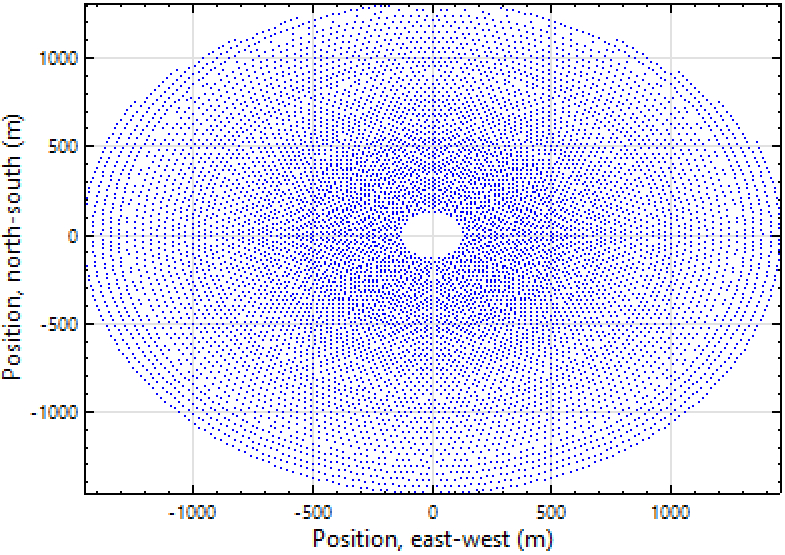
\includegraphics[width=0.95\textwidth]{FIG/SM20}
                \caption{SM:~2.0}\label{SM2.0}
        \end{subfigure}%
        ~
        \begin{subfigure}[b]{0.5\textwidth}
                \centering
                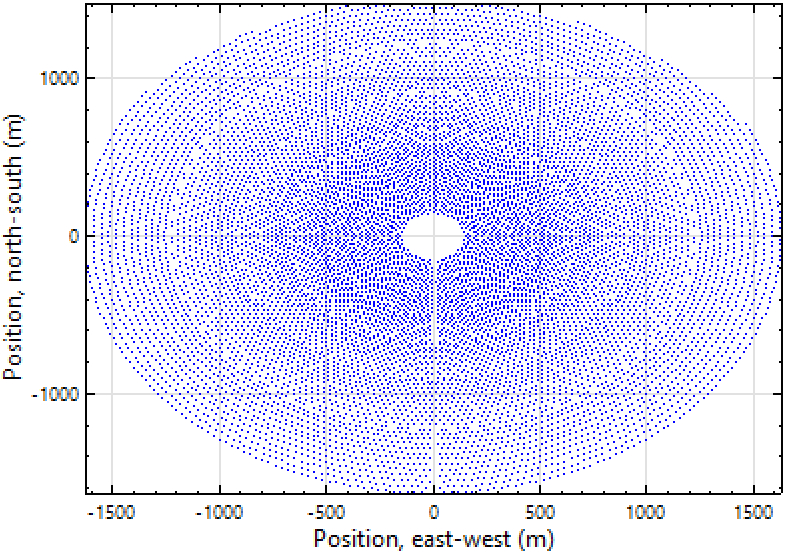
\includegraphics[width=0.95\textwidth]{FIG/SM25}
                \caption{SM:~2.5}\label{SM2.5}
        \end{subfigure}
        
\par\medskip % Linebreak
                
        \begin{subfigure}[b]{0.5\textwidth}
                \centering
                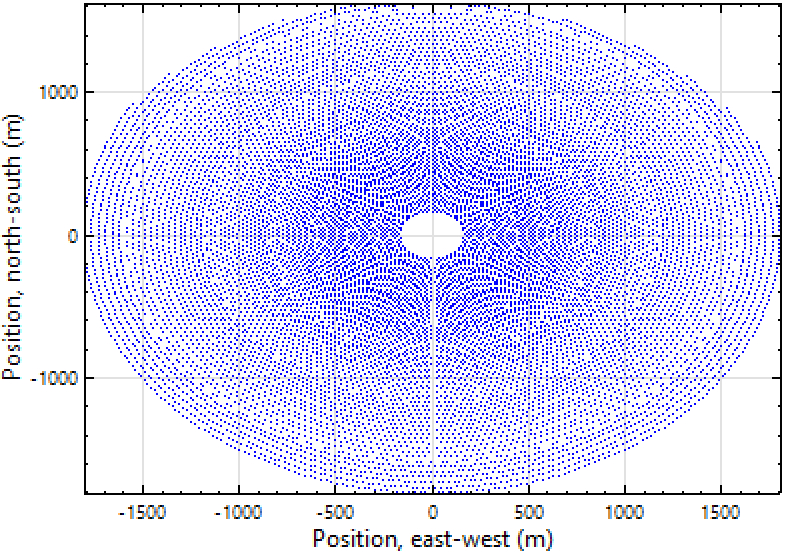
\includegraphics[width=0.95\textwidth]{FIG/SM30}
                \caption{SM:~3.0}\label{SM3.0}
        \end{subfigure}%
        ~
        \begin{subfigure}[b]{0.5\textwidth}
                \centering
                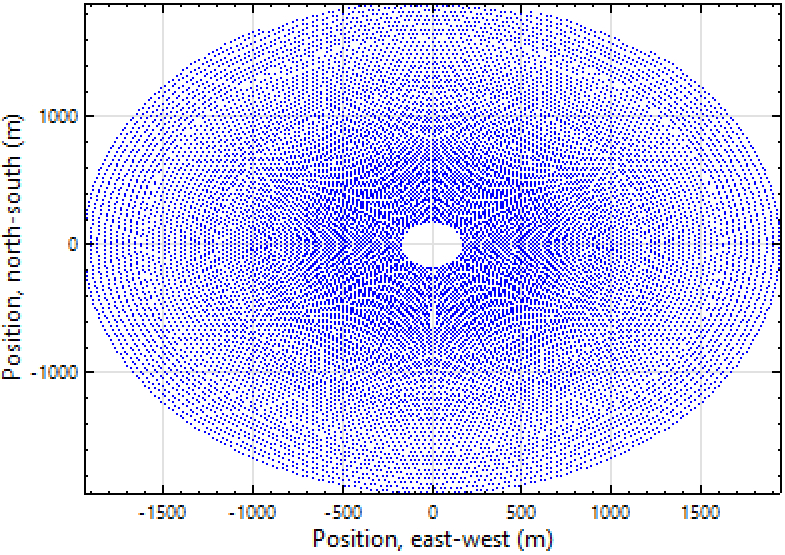
\includegraphics[width=0.95\textwidth]{FIG/SM35}
                \caption{SM:~3.5}\label{SM3.5}
        \end{subfigure}
        \caption[Simulated heliostat field layout at diferent solar multiples (SM).]{Simulated heliostat field layout at diferent solar multiples (SM).}\label{SM}
\end{figure}

\begin{figure}[htbp]  
\centering
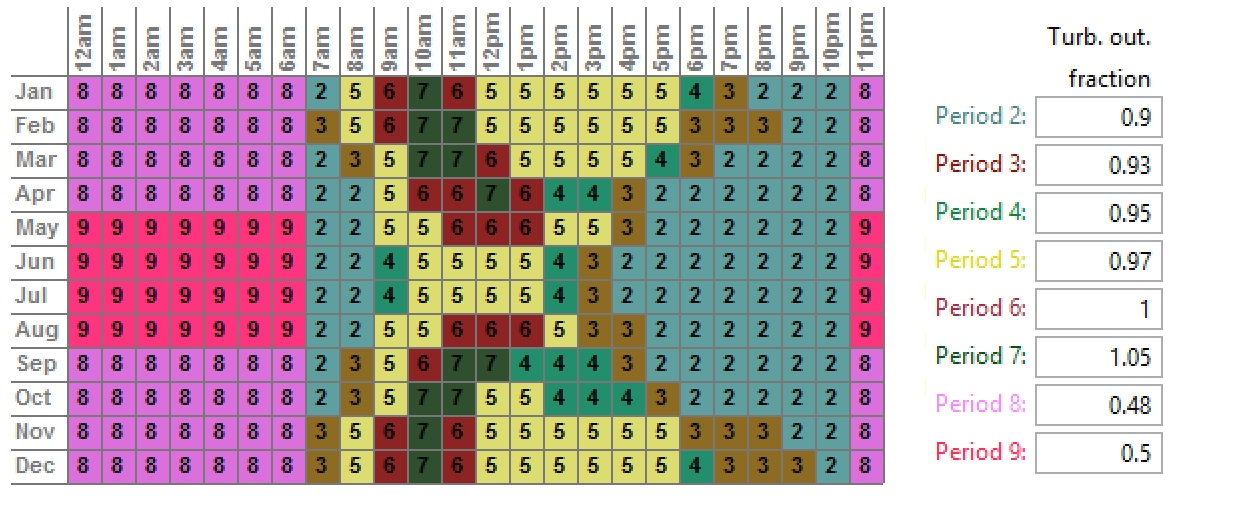
\includegraphics[width=0.95\linewidth]{FIG/CR_turbineoutput}
\caption[TES dispatch control matrix for turbine output fraction of CR simulation in SAM.]{TES dispatch control matrix for turbine output fraction of CR simulation in SAM.}\label{CR_turbineoutput}
\end{figure}
\pagebreak
\section{PTC system simulation design documentary}\label{PTCdocumentary}

\begin{figure}[bhtp]
\centering
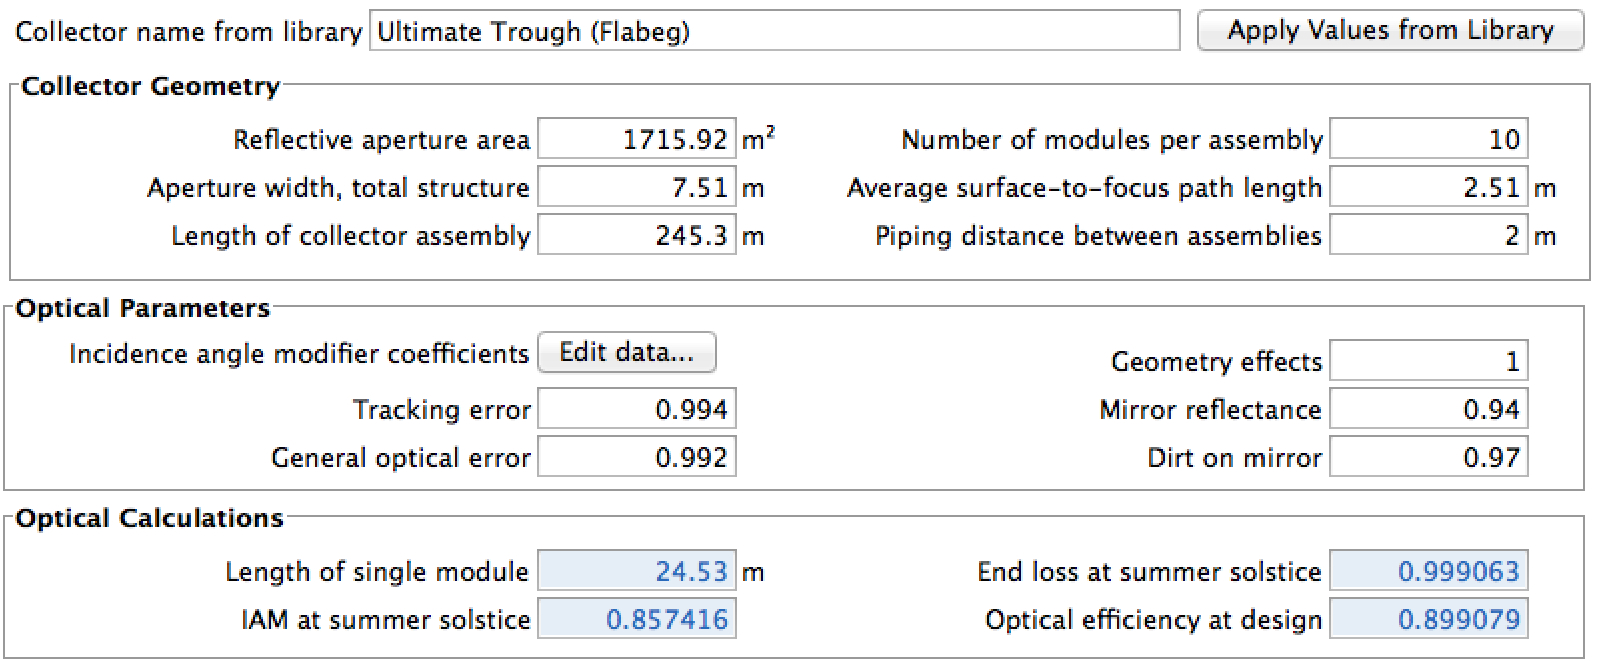
\includegraphics[width=0.95\linewidth]{FIG/PTC_Ultimate_config}
\caption[Screenshot of Ultimate Trough SCA input parameter for SAM.]{Screenshot of Ultimate Trough SCA input parameter for SAM.}\label{PTC_Ultimate_config}
\end{figure}

\begin{figure}[htbp]  
\centering
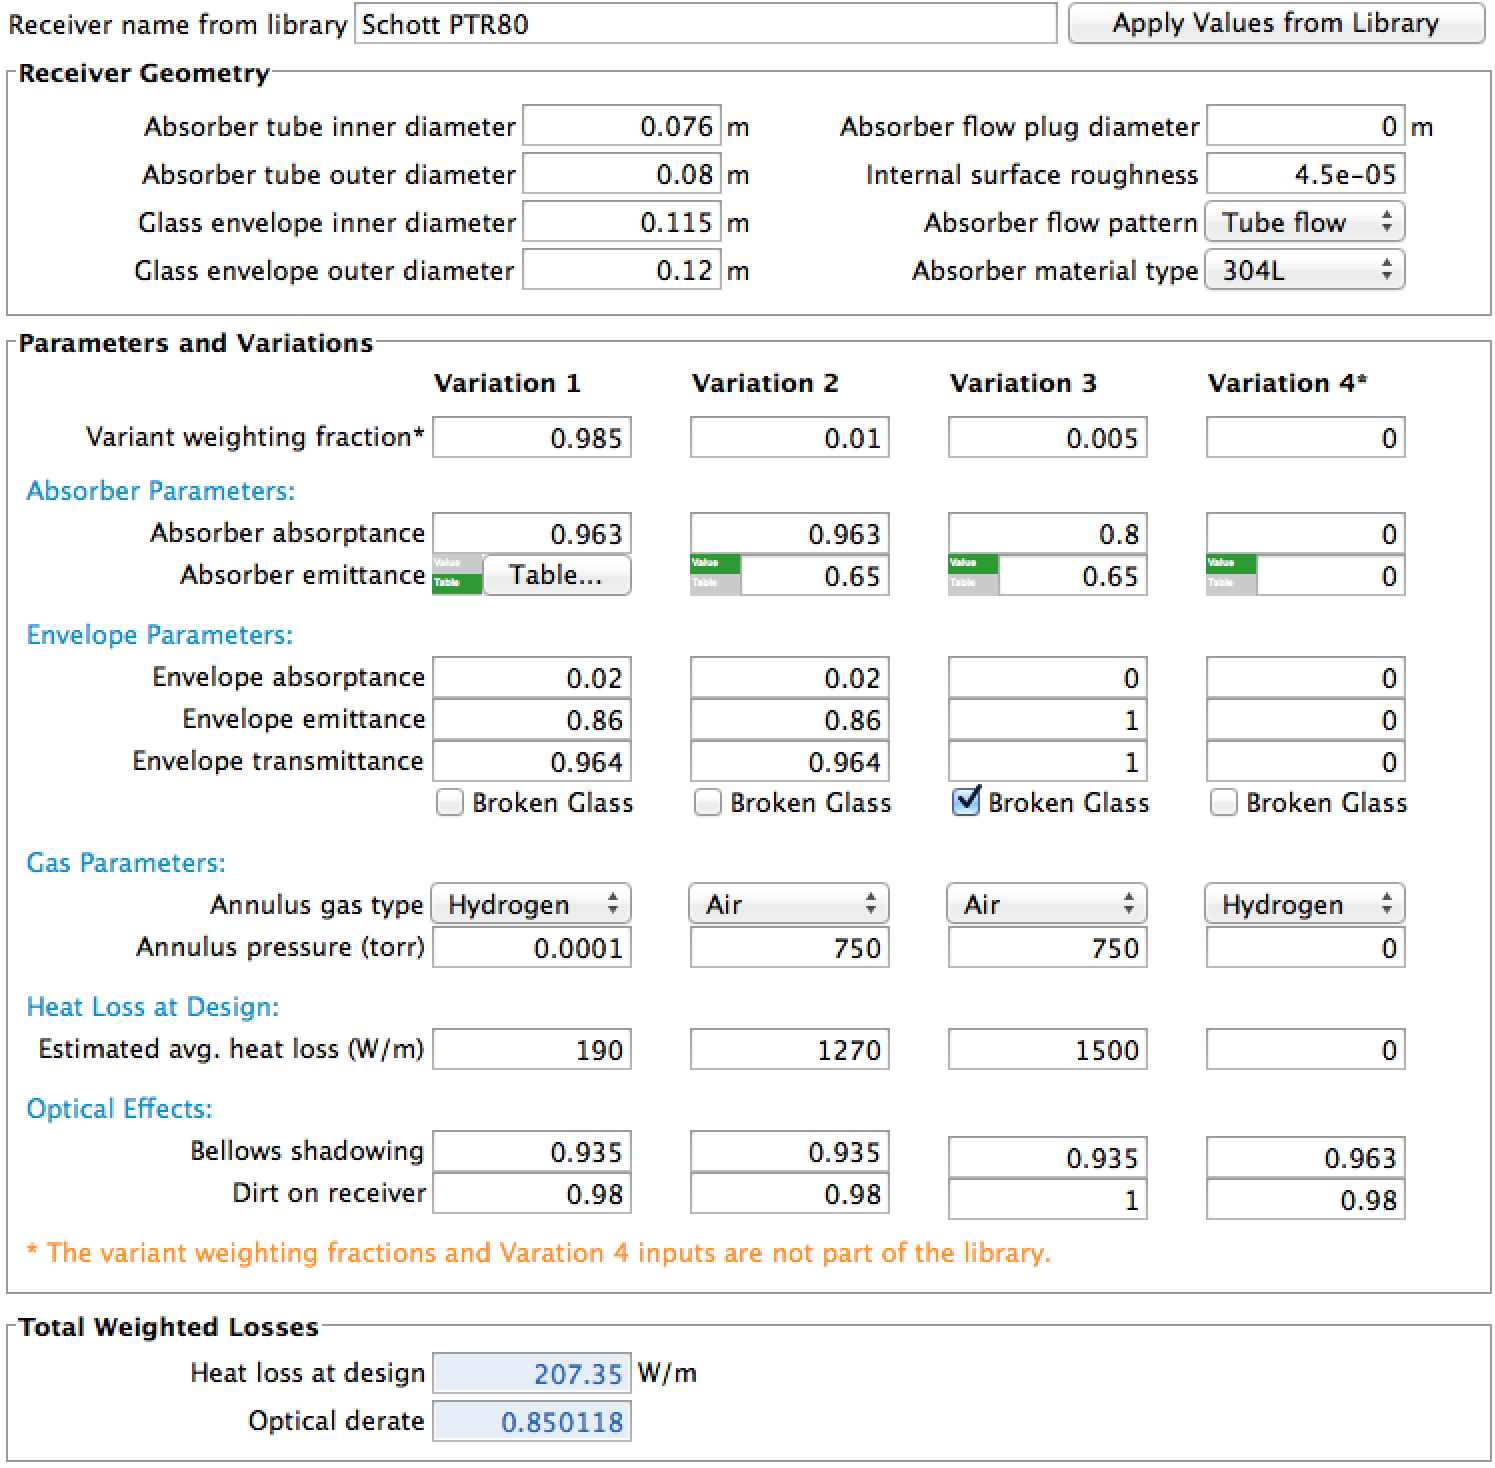
\includegraphics[width=0.95\linewidth]{FIG/PTC_HCE}
\caption[Screenshot of Schott PTR80 input parameter for SAM.]{Screenshot of Schott PTR80 input parameter for SAM, based on data from \cite{Kutscher2012}.}\label{PTC_HCE}
\end{figure}

\begin{figure}[htbp]  
\centering
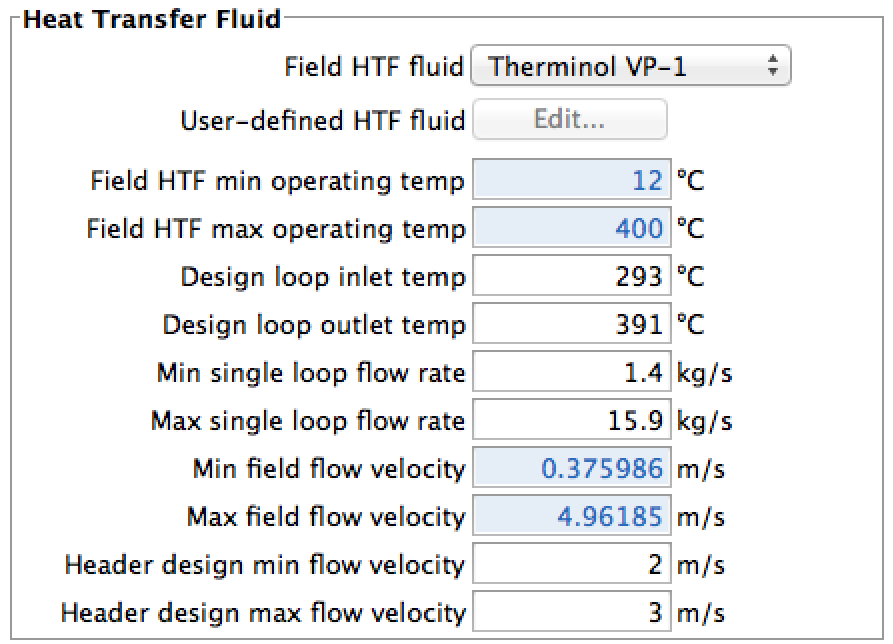
\includegraphics[width=0.6\linewidth]{FIG/PTC_HTF}
\caption[Screenshot of HTF input parameter for SAM.]{Screenshot of HTF input parameter for SAM.}\label{PTC_HTF}
\end{figure}

\begin{figure}[htbp]  
\centering
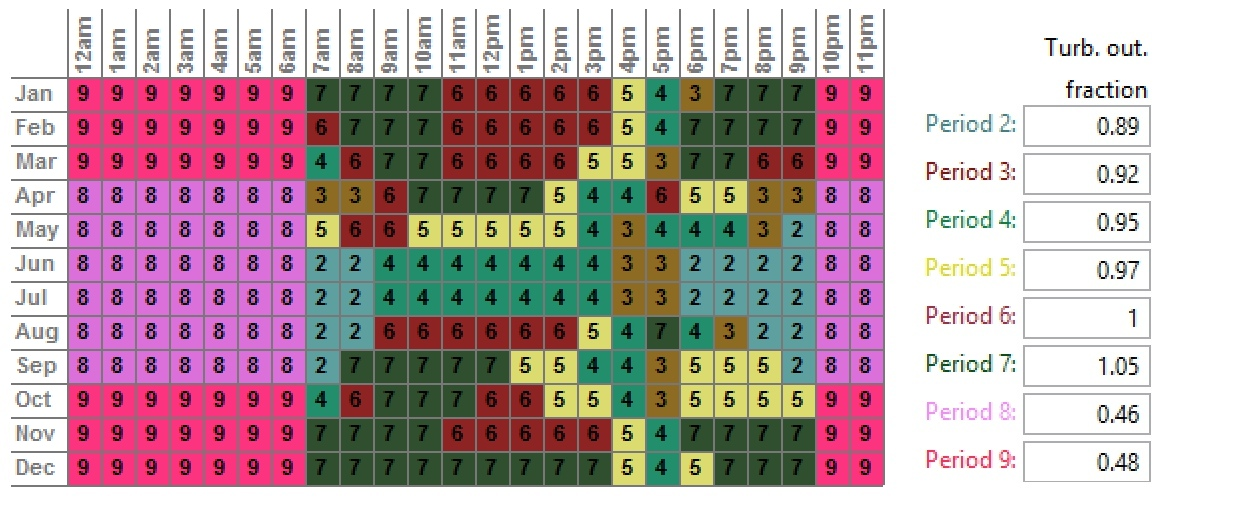
\includegraphics[width=0.95\linewidth]{FIG/PTC_turbineoutput}
\caption[TES dispatch control matrix for turbine output fraction of PTC simulation in SAM.]{TES dispatch control matrix for turbine output fraction of PTC simulation in SAM.}\label{PTC_turbineoutput}
\end{figure}
\pagebreak
\section{PV system simulation design documentary}\label{PVdocumentary}

\begin{table}[htbp]  
  \centering
	\begin{tabular}{  p{5.0cm}  C{5.0cm}  C{1.4cm} } 
	\hline	
\textbf{Item} & \textbf{Value} & \textbf{Unit} \\ \hline \hline
Manufacturer  & BYD COMPANY LIMITED & - \\ 
Model & BYD 305P6C-36 & - \\ 
Cell type &  poly-crystalline silicon & - \\ \hline
Maximum power & 304.99 & \si{\wattel} \\ 
Nominal efficiency & 15.72 & \si{\percent} \\ 
Maximum power voltage & 36.2 & \si{\voltsdc} \\ 
Maximum power current & 8.4 & \si{\ampsdc}  \\
Open circuit voltage & 45.5 & \si{\voltsdc}  \\ 
Short circuit current & 8.9 & \si{\ampsdc}  \\
Temperature efficiency & -0.41 & \si{\percent\celsius}\\
Module area & 1.94 & \si{\square\metre} \\ 
Number of cells & 72 & -\\
\hline
\end{tabular}
\caption[Module specification of BYD 305P6C-36.]{Module specification of BYD 305P6C-36 under STC: \SI{1000}{\watt\per\square\metre}, cell temperature \SI{25}{\celsius} \cite{NREL2015g}.}\label{tbl: PVmodule}
\end{table}

\begin{figure}[htbp]  
\centering
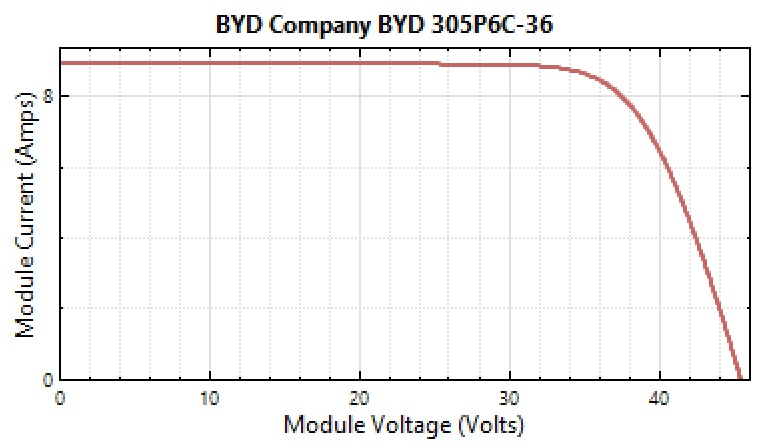
\includegraphics[width=0.70\linewidth]{FIG/PVModuleVA}
\caption[Current–voltage characteristic under STC of module BYD 305P6C-36.]{Current–voltage characteristic under STC of module BYD 305P6C-36 \cite{NREL2015g}.}\label{PVModuleVA}
\end{figure}

\begin{figure}[htbp]  
\centering
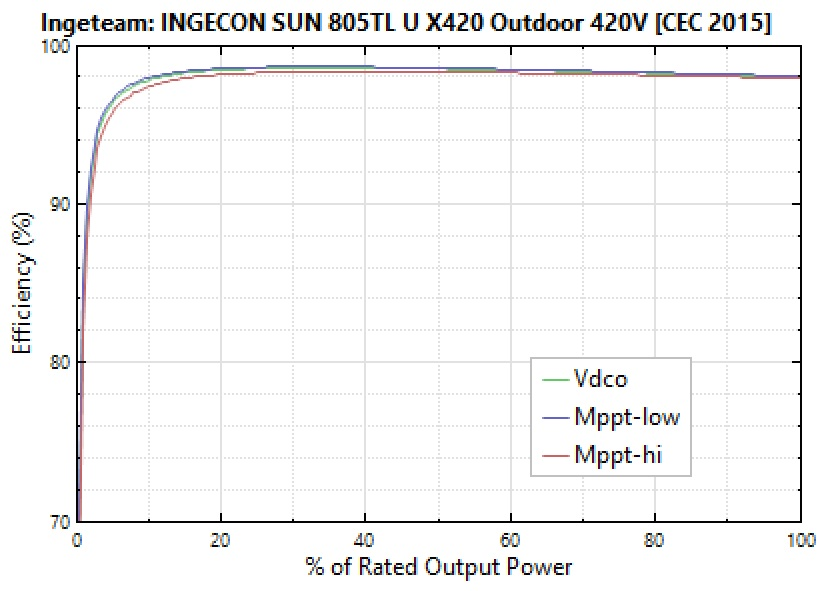
\includegraphics[width=0.75\linewidth]{FIG/InverterEfficiencyCurve}
\caption[Efficientcy characteristic of Ingecon Sun 805TL U X420 Outdoor.]{Efficientcy characteristic of Ingecon Sun 805TL U X420 Outdoor \cite{IngeteamINC.2015,NREL2015g}.}\label{InverterEfficiencyCurve}
\end{figure}

\begin{table}[htbp]  
  \centering
	\begin{tabular}{ p{6.0cm}  C{7.0cm}  C{1.5cm} } 
	\hline	
\textbf{Item} & \textbf{Value} & \textbf{Unit} \\ \hline \hline
Manufacturer  & Ingeteam Power Technology & - \\ 
Model & Ingecon Sun 805TL U X420 Outdoor & - \\ 
Type &  central inverter & - \\ \hline
\textbf{Input (dc)} &  &  \\ 
Maximum power & 821.39 & kW\textsubscript{dc} \\ 
Voltage range & 611-820 & V\textsubscript{dc} \\ 
Maximum voltage & 1~000 & V\textsubscript{dc} \\ 
Maximum current & 1~350 & A\textsubscript{dc} \\
Nominal voltage & 715.91 & V\textsubscript{dc} \\ \hline
\textbf{Output (ac)} &  &  \\ 
Maximum power & 805 & kW\textsubscript{ac} \\ 
Nominal voltage & 420 & V\textsubscript{ac} \\
Maximum current & 1.35 & A\textsubscript{ac} \\
Frequency & 50-60 & Hz \\
cos$\phi$ & 1 & -\\ \hline
Maximum efficiency & 98.33 & \\% 
European efficiency & 98.29 & \\% 
Power consumption in operation &1.25 & kW\textsubscript{dc} \\ 
Power consumption at night & 0.12 & kW\textsubscript{ac} \\ 
\hline
\end{tabular}
\caption[Inverter specifications of Ingecon Sun 805TL U X420 Outdoor.]{Inverter specifications of Ingecon Sun 805TL U X420 Outdoor \cite{IngeteamINC.2015,NREL2015g}.}\label{tbl: PVinverter}
\end{table}

\begin{figure}[!htbp]  
\centering
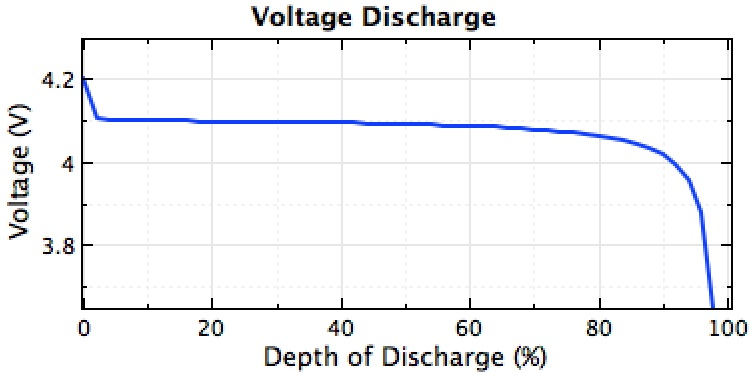
\includegraphics[width=0.6\linewidth]{FIG/EES_VoltageDischarge}
\caption[Voltage proparties of NCA Li-Ion battery.]{Voltage proparties of NCA Li-Ion battery..}\label{EES_VoltageDischarge}
\end{figure}

\pagebreak